\section{近邻体系与可迁移变量}

\begin{figure}[t]
  \centering
  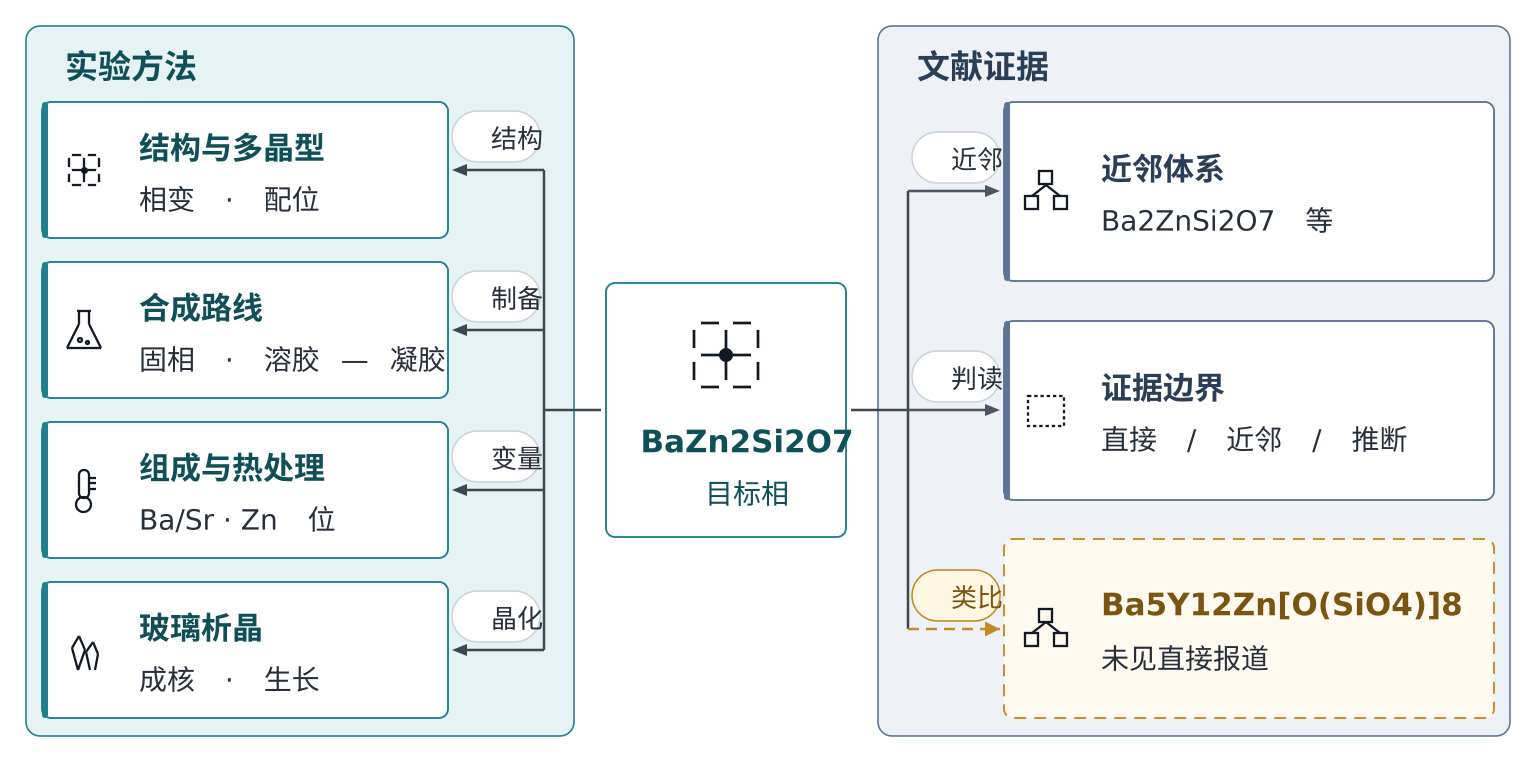
\includegraphics[width=0.9\linewidth]{../figures/svg/taxonomy_phase_control.svg}
  \caption{BaZn$_2$Si$_2$O$_7$ 合成与相控制分类框架。实线分支为目标相直接或近邻实验依据，虚线节点为尚缺直接结构报道的比较对象。}
  \label{fig:taxonomy}
\end{figure}

\subsection{Ba/Sr 替位}

Ba$_{1-x}$Sr$_x$Zn$_2$Si$_2$O$_7$ 是最成熟的同型近邻。Sr$^{2+}$ 取代 Ba$^{2+}$ 会降低高温相的形成温度；当替位超过约 10\% 时，高温结构可在室温保留，并表现为近零或负热膨胀 \cite{thieme2015ba1,thieme2016very,thieme2017variable,zou2021near}。单晶衍射将稳定相确定为正交 Cmcm，ZnO$_4$ 链的扭曲和摆动被认为是负热膨胀的重要结构来源 \cite{thieme2015ba1}。这说明 A 位尺寸和多面体空隙是相控制的有效旋钮，但不能直接推断 Y$^{3+}$ 大量进入同一位点。

\subsection{Zn 位与 Si 位替位}

Mg、Co、Mn、Ni、Cu 等二价离子可在不同范围替代 Zn。替位量超过临界值时，低温结构可能重新出现，显示局域配位偏好与长程相稳定性之间存在竞争 \cite{thieme2016new,kerstan2013bazn2si2o7}。Ge 替 Si 则通过四面体尺寸和键柔性改变相变温度；Sr-free 组成的 Ge 固溶度有限，而含 Sr 组成可保持高温结构至更高 Ge 含量 \cite{thieme2016negative}。

\subsection{玻璃—陶瓷工艺}

玻璃路线研究揭示了与化学组成同等重要的动力学因素。Pt 成核剂促进异质成核，Nb$_2$O$_5$/Ta$_2$O$_5$ 使表面和体析晶比例发生变化，贵金属还可能形成合金或核壳结构 \cite{vladislavova2017heterogeneous,heitmann2019surface,thieme2022noble,thieme2018growth}。晶粒尺寸低于约 80~$\mu$m 时，微裂纹减少，宏观膨胀更接近晶体本征值 \cite{thieme2016thermal}。因此，对 BaZn$_2$Si$_2$O$_7$ 的“相控制”应同时报告相组成、晶粒尺度和裂纹状态。
